% Elsevier CAS 2.4 from the template archive supplied by the author.
% CAS title notes are metadata, without ordinary footnote hyperlink anchors.
\PassOptionsToPackage{hyperfootnotes=false}{hyperref}
\ifdefined\KBSReview
  \documentclass[a4paper,fleqn,review]{cas-sc}
\else
  \documentclass[a4paper,fleqn]{cas-dc}
\fi
\usepackage[numbers,sort&compress]{natbib}
\newenvironment{kbsmalltable}{\begin{table}[pos=htbp]}{\end{table}}
\usepackage{microtype}
\usepackage{amsmath,amssymb,amsthm}
\usepackage{booktabs,graphicx,array,adjustbox,placeins}
\usepackage{xurl,hyperref,enumitem}
\setlength{\emergencystretch}{3em}
\hypersetup{hidelinks,pdftitle={Supplementary Development Evidence for Compact Rule Distillation},pdfauthor={Xu Wang and Zhiqiang Chen}}
% Preserve CAS headers and pagination without claiming submission or acceptance.
\ExplSyntaxOn
\keys_set:nn { stm / mktitle } { nologo = true }
% CAS 2.4 prints an empty ORCID note unless the caller guards it.
\cs_new_eq:NN \kbs_print_orcid: \printorcid
\RenewDocumentCommand \printorcid { }
  { \seq_if_empty:NF \g_stm_orcid_seq { \kbs_print_orcid: } }
% The keyword panel is intentionally overlaid in a zero-width box.
% Flexible trailing space makes that overlay explicit to TeX's box checker.
\expandafter\patchcmd\csname environment~Abstract~code\endcsname
  { \box \g_stm_key_box } { \box \g_stm_key_box \hss }
  { } { \PackageError{KBS}{CAS~keyword~panel~patch~failed}{Use~the~bundled~CAS~2.4~files.} }
\cs_set:Npn \__first_footerline:
  {\small\rmfamily\itshape Manuscript~prepared~for~Knowledge-Based~Systems}
\ExplSyntaxOff
\makeatletter
% Keep float-only pages aligned at the top, with consistent table spacing.
\setlength{\@fptop}{0pt}
\setlength{\@fpsep}{12pt}
\setlength{\@fpbot}{0pt plus 1fil}
\setlength{\@dblfptop}{0pt}
\setlength{\@dblfpsep}{12pt}
\setlength{\@dblfpbot}{0pt plus 1fil}
\makeatother
\ifdefined\KBSReview
  \newenvironment{kbtable}{\begin{table}[pos=htbp]}{\end{table}}
  \newenvironment{kbfigure}{\begin{figure}[pos=htbp]}{\end{figure}}
  \newcommand{\kbsbarrier}{\FloatBarrier}
\else
  \newenvironment{kbtable}{\begin{table*}[pos=!tp,width=\textwidth]}{\end{table*}}
  \newenvironment{kbfigure}{\begin{figure*}[pos=t,width=\textwidth]}{\end{figure*}}
  \newcommand{\kbsbarrier}{}
\fi
\setcounter{dbltopnumber}{4}
\renewcommand{\dbltopfraction}{0.9}
\renewcommand{\dblfloatpagefraction}{0.6}
\renewcommand{\textfraction}{0.1}
\newtheorem{proposition}{Proposition}
\newcommand{\method}{Refined LFIO}
\newcommand{\evidence}{docs/research/paper_2026-09-24}
\newcommand{\RefinedFidelityClean}{93.08}
\newcommand{\RefinedConditionsClean}{14.075}
\newcommand{\RuleFitFidelityClean}{94.00}
\newcommand{\RuleFitConditionsClean}{55.150}
\newcommand{\RefinedBAClean}{86.50}
\newcommand{\RefinedFidelityNoisy}{88.82}
\newcommand{\RefinedConditionsNoisy}{14.600}
\newcommand{\RuleFitFidelityNoisy}{89.12}
\newcommand{\RuleFitConditionsNoisy}{55.950}
\newcommand{\RefinedBANoisy}{83.95}
\newcommand{\DistillPredictionStability}{89.42}
\newcommand{\DistillFeatureStability}{0.446}
\newcommand{\DistillRuleStability}{0.219}
\newcommand{\BudgetEightClean}{92.89}
\newcommand{\RipperEightClean}{90.37}
\newcommand{\BudgetRipperMean}{2.52}
\newcommand{\BudgetRipperLow}{0.70}
\newcommand{\BudgetRipperHigh}{4.62}
\newcommand{\TTEightFeasible}{3}
\newcommand{\NeuEightFeasible}{10}
\newcommand{\TTThirtyTwoFeasible}{21}
\newcommand{\NeuThirtyTwoFeasible}{39}
\newcommand{\BudgetEightNoisy}{88.91}
\newcommand{\RipperEightNoisy}{86.88}
\newcommand{\MajorityOldGap}{30.11}
\newcommand{\MajorityNewGap}{2.61}
\newcommand{\MajorityOldOptimal}{2}
\newcommand{\MajorityNewOptimal}{29}
\newcommand{\MajorityCertified}{48}
\newcommand{\ParityOldGap}{24.08}
\newcommand{\ParityNewGap}{21.17}
\newcommand{\ParityOldOptimal}{10}
\newcommand{\ParityNewOptimal}{14}
\newcommand{\ParityCertified}{45}
\newcommand{\CertifiedSettings}{141}
\newcommand{\ImprovedSettings}{56}
\newcommand{\ExternalRefinedClean}{81.32}
\newcommand{\ExternalRipperClean}{73.55}
\newcommand{\ExternalGainCleanMean}{0.48}
\newcommand{\ExternalGainCleanLow}{-0.11}
\newcommand{\ExternalGainCleanHigh}{1.12}
\newcommand{\ExternalRefinedNoisy}{71.30}
\newcommand{\ExternalRipperNoisy}{67.38}
\newcommand{\ExternalGainNoisyMean}{1.75}
\newcommand{\ExternalGainNoisyLow}{0.28}
\newcommand{\ExternalGainNoisyHigh}{3.47}

\newcommand{\RuleFitFourFeasibleClean}{48}
\newcommand{\NewTeacherBAClean}{75.80}
\newcommand{\NewRefinedBAClean}{74.19}
\newcommand{\RuleFitFourFeasibleNoisy}{46}
\newcommand{\NewTeacherBANoisy}{71.65}
\newcommand{\NewRefinedBANoisy}{72.51}
\newcommand{\NewRefinedClean}{91.10}
\newcommand{\NewRefinedNoisy}{87.05}
\newcommand{\NewBRCGClean}{90.96}
\newcommand{\NewBRCGNoisy}{85.61}
\newcommand{\NewTreeClean}{81.36}
\newcommand{\NewTreeNoisy}{79.83}
\newcommand{\NewRipperClean}{88.56}
\newcommand{\NewRipperNoisy}{84.94}

\newcommand{\FollowMedianClean}{79.80}
\newcommand{\FollowQuantileClean}{83.19}
\newcommand{\FollowBRCGClean}{84.11}
\newcommand{\FollowMedianNoisy}{75.77}
\newcommand{\FollowQuantileNoisy}{79.06}
\newcommand{\FollowBRCGNoisy}{79.91}

\begin{document}
\shorttitle{Development Evidence}
\shortauthors{Xu Wang and Zhiqiang Chen}
\title[mode=title]{Supplementary Development Evidence for Compact Rule Distillation}
\author[1,2,3]{Xu Wang}
\cormark[1]
\ead{xwang@idt.eitech.edu.cn}
\author[1,2,3]{Zhiqiang Chen}
\ead{zqchen@idt.eitech.edu.cn}
\cortext[1]{Corresponding author.}
\affiliation[1]{organization={Ningbo Institute of Digital Twin, Eastern Institute of Technology},city={Ningbo},postcode={315200},state={Zhejiang},country={P.R. China}}
\affiliation[2]{organization={Ningbo Key Laboratory of Spatial Intelligence and Digital Derivative},city={Ningbo},postcode={315200},state={Zhejiang},country={P.R. China}}
\affiliation[3]{organization={Zhejiang Key Laboratory of Industrial Intelligence and Digital Twin},city={Ningbo},postcode={315200},state={Zhejiang},country={P.R. China}}
\begin{abstract}
This supplement preserves the development evidence that preceded the independent numerical-teacher extension. Refined LFIO denotes the earlier extractor. Its search ablations, synthetic certificates, ten-dataset comparisons, neural Boolean-input adaptations, numerical-vocabulary follow-ups, and retrospective encoding analysis are retained with their original scopes. Their primary endpoints are local to these earlier protocols. They are not pooled with the independent six-dataset study in the main article and do not establish the effectiveness of its later diagnostic allocation policy.
\end{abstract}
\begin{keywords}Rule distillation \sep Development evidence \sep Reproducibility\end{keywords}
\maketitle
% CAS replaces PDF author metadata while creating its title block.
\hypersetup{pdfauthor={Xu Wang and Zhiqiang Chen}}
\section{Scope and chronology}
The initial extension, validation-opportunity follow-up, and scored-work/MDL extension were fixed successively in September 2026. The empirical encoding-ceiling reanalysis was added on 15 October. This material informed the subsequent independent-cohort protocol; new split seeds in these development studies do not create new datasets. The main article supersedes the earlier framing and reports the later Diagnostic LFIO controller. The historical search heuristic is kept executable and unchanged.
\section{Budget-constrained Boolean distillation}
\subsection{Representation and targets}
Let $X\in\{0,1\}^{n\times d}$ contain complete Boolean observations. Each body $r$ is a conjunction of distinct-feature literals $(j,v)$, $v\in\{0,1\}$. All selected bodies share head $h$. With $C_R(x)=\bigvee_{r\in R}r(x)$, prediction is
\begin{equation}
 f_{R,h}(x)=\begin{cases}h,& C_R(x)=1,\\1-h,&C_R(x)=0.\end{cases}
\end{equation}
The exported default class $1-h$ is part of the model. An empty program predicts that class. Rule size is $L(R)=\sum_{r\in R}|r|$, and a condition budget requires $L(R)\leq B$. Unconstrained experiments omit this hard ceiling while retaining length regularization and a 32-body limit.

For distillation, a teacher $g$ is fitted only on the fitting partition. Its hard predictions on fitting and validation observations are the surrogate targets. Selection uses validation balanced accuracy against the teacher; final fidelity is ordinary agreement with the teacher on held-out test observations. Ground-truth balanced accuracy is reported separately. Direct-label experiments instead use the observed, possibly corrupted, fitting and validation labels. Missing values, relations, recursion, and open-world or default-negation semantics are outside this propositional model.

\subsection{Candidate pool and objective}
Training coverage of each literal is stored as a packed bit vector. Intersections give conjunction coverage, and unions give program coverage. We enumerate all distinct conjunctions through complete depth levels, subject to
\begin{equation}
 \sum_{\ell=1}^{D}\binom d\ell 2^\ell\leq 50{,}000,
\end{equation}
and retain bodies covering at least three fitting observations. Requested depths are $1,\ldots,5$. The complete-level policy avoids privileging low-index features, but restricts maximum feasible depth to 3, 4, 2, and 2 for breast cancer, banknote, ionosphere, and spambase, respectively.

For fixed $h$, define $P=\{i:y_i=h\}$ and $N=\{i:y_i\ne h\}$. When both classes occur, $w_P=n/(2|P|)$ and $w_N=n/(2|N|)$. The training objective is
\begin{equation}\label{eq:objective}
 \begin{aligned}
 J(R;h,\alpha)={}&w_P|P\setminus C_R|+w_N|N\cap C_R|\\
    &+\alpha\log_2(n)\sum_{r\in R}(|r|+1).
 \end{aligned}
\end{equation}
The error terms equal $n$ times balanced error; the penalty charges both conditions and bodies. Feature identities are not encoded, so this is not a formal MDL code~\citep{rissanen1978}. Single-class fitting targets use a constant predictor.

For candidate $r$, the gain from adding its coverage to the current union is
\begin{equation}\label{eq:gain}
 \begin{aligned}
 \Delta(r)={}&w_P|C_r\cap(P\setminus C_R)|\\
 &-w_N|C_r\cap(N\setminus C_R)|\\
 &-\alpha\log_2(n)(|r|+1).
 \end{aligned}
\end{equation}
Only newly corrected or newly incorrect observations contribute. Thus overlapping bodies cannot receive duplicate credit.

The implementation prepares the supported candidate pool once for repeated budget fits on identical fitting inputs. A fingerprint checks the Boolean matrix and enumeration configuration before reuse. This cache changes neither the candidate space nor the selected predictor. Candidate coverage requires $O(M\lceil n/w\rceil)$ machine words for $M$ retained bodies and word width $w$. A greedy pass scans the pool; a repair iteration evaluates additions and up to $|R|$ replacement neighborhoods. Consequently, repair can dominate computation even when the final explanation is short. Candidate visits and complete-grid fitting times are reported separately from model size.

\subsection{Two starts and bounded repair}\label{sec:search}
For every feasible depth, head $h\in\{0,1\}$, and $\alpha\in\{0,0.05,0.2,0.8\}$, the procedure is:
\begin{enumerate}[leftmargin=*,itemsep=3pt]
\item \textbf{Independent starts.} Fit an ordinary greedy program from the full candidate pool and a second program from candidates satisfying $C_r\cap N=\varnothing$. The latter is pure with respect to the observed training targets and chosen head, not necessarily class one or the unknown concept. Each start repeatedly adds the largest positive-gain body within the size and rule-count limits, then repeatedly deletes a body if this does not increase $J$.
\item \textbf{Repair.} For each distinct initial program, search the full pool for an addition, deletion, or one-for-one replacement. At each iteration choose the move with the lowest resulting union-based objective; at equal objective accept a move only if it reduces total conditions, then rule count. Stop when no acceptable move exists or after eight iterations. Prefix/suffix coverage unions compute coverage after removing a body. All moves respect $B$ and the 32-body cap.
\item \textbf{Validation candidates.} Retain both the initial program and its final repaired version when repair makes a move. Identical initial programs are evaluated once. Intermediate repair steps are not additional validation candidates.
\item \textbf{Selection.} Maximize validation balanced accuracy, breaking ties by fewer conditions, fewer bodies, shallower depth, larger penalty, and head zero. Exact remaining ties retain the first enumerated candidate. The selected program is not refitted on the validation partition.
\end{enumerate}
Purity is an initialization restriction only; repair may introduce an impure body if it improves the objective. Conversely, validation can retain an initial program despite an improved training objective. This guards against assuming that every local repair improves generalization. The factorial ablation disables either component or both within the same implementation and selection grid. Disabling both retains ordinary greedy construction and backward deletion.

\begin{proposition}[Exact replacement criterion]
For a replacement of $r\in R$ by $s\notin R\setminus\{r\}$, let $R_-=R\setminus\{r\}$, $A=C_s\setminus C_{R_-}$, $D=C_r\setminus C_{R_-}$, $G=A\setminus D$, and $H=D\setminus A$. With $\lambda=\alpha\log_2 n$, the replacement strictly improves the training objective exactly when
\begin{equation}
\begin{aligned}
&w_P|P\cap G|+w_N|N\cap H|\\
&\quad >w_N|N\cap G|+w_P|P\cap H|\\
&\qquad +\lambda(|s|-|r|).
\end{aligned}
\end{equation}
\end{proposition}
\begin{proof}
Only newly covered observations $G$ and no-longer-covered observations $H$ change prediction. Correcting a missed head observation in $G$ saves $w_P$; retracting a false head observation in $H$ saves $w_N$. The other two transitions incur the corresponding weights. The body count is unchanged, leaving the condition-length penalty difference shown above.
\end{proof}
This identity explains the move criterion without an approximation or generalization guarantee. In particular, addition alone has no retracted-coverage term. At a saturated condition budget, replacement can recover false head predictions while staying feasible. Section~\ref{sec:cases} shows that this training improvement may help or hurt held-out fidelity.

Accepted greedy moves reduce the objective; deletion and repair do not increase it, up to recorded floating-point tolerances. Equal-objective repair reduces conditions and then body count. Finite grids, at most 32 greedy additions, and at most eight repair moves ensure termination. A program stopped at the iteration cap need not be a local optimum.

\begin{proposition}[Parity capacity]
Exact $d$-variable parity in this single-head language requires full-depth satisfiable bodies and at least $2^{d-1}$ bodies, hence at least $d2^{d-1}$ condition occurrences.
\end{proposition}
\begin{proof}
If a body omits a variable, flipping that variable preserves the body and changes parity, so the body covers the wrong head class. A full-depth body covers one assignment; either parity class contains $2^{d-1}$ assignments.
\end{proof}
Five-bit parity therefore needs 16 bodies and 80 conditions. A smaller depth or condition ceiling excludes an exact solution irrespective of teacher quality. When the language admits the solution, search can still fail; Section~\ref{sec:diagnostics} tests that distinction.

\subsection{An empirical ceiling for a fixed vocabulary}\label{sec:vocabulary-ceiling}
Let $\phi(x)$ be the Boolean encoding supplied to a student and let $S$ be a fixed nonempty sample of $n$ observations with binary teacher outputs. For each observed encoding $z$, let $n_{z,c}=|\{i:\phi(x_i)=z,\ g(x_i)=c\}|$.
\begin{proposition}[Empirical vocabulary ceiling]\label{prop:vocabulary}
The largest empirical fidelity of any deterministic function of $\phi(x)$ is
\begin{equation}\label{eq:vocabulary-ceiling}
 F^\star_\phi(S)=\frac{1}{n}\sum_z\max(n_{z,0},n_{z,1})
 =1-\frac{1}{n}\sum_z\min(n_{z,0},n_{z,1}).
\end{equation}
Every budget-constrained rule student of this encoding has fidelity at most $F^\star_\phi(S)$. If $\phi'$ retains all predicates of $\phi$, then $F^\star_{\phi'}(S)\geq F^\star_\phi(S)$ on the same sample and teacher.
\end{proposition}
\begin{proof}
A deterministic student gives the same prediction to all observations with encoding $z$, so it can agree with at most the larger of the two teacher-label counts. Choosing each group's majority attains their sum. Retaining predicates only partitions existing groups into finer groups; their separate majority counts sum to at least the previous majority count.
\end{proof}
This elementary empirical majority-decoding identity supplies a vocabulary diagnostic, without fitting another student. Conflicting teacher outputs within one encoding prove information loss that more search cannot recover. The unrestricted decoder attaining the bound may require a large rule program, so a high ceiling does not establish feasibility under a condition or depth limit. On a test sample, the ceiling uses test teacher outputs retrospectively and is not an estimate of achievable population fidelity. It can be vacuous when encoded patterns are unique. Moreover, distance from this ceiling combines language capacity, fitting, and selection effects; only a matched optimization oracle can certify a training search gap. The objective in Equation~\ref{eq:objective} additionally uses balanced weights and a length penalty, whereas this ceiling concerns ordinary fidelity.

\subsection{Fitting numerical predicates}
For a numerical feature $x_j$, a fitting-only quantile $\widehat Q_{j,q}$ defines $z_{j,q}(x)=\mathbf{1}[x_j>\widehat Q_{j,q}]$. The original vocabulary uses $q=0.5$; the numerical follow-up uses $q\in\{0.25,0.5,0.75\}$, removing duplicate threshold values within a feature. The median vocabulary is therefore nested in the richer vocabulary. Neither validation nor test observations determine thresholds. Both the greater-than test and its complementary less-than-or-equal test are executable predicates. An interval requiring two threshold tests consumes two conditions. This preprocessing extends the available vocabulary while leaving Refined LFIO's objective and search unchanged.

The supervised extension retains each median and adds at most two cuts informed by fitting teacher labels. It applies the established entropy/MDL criterion of Fayyad and Irani~\citep{fayyad1993}. For an interval $S$ of $n$ fitting observations, choose the distinct-value boundary $t$ with largest information gain $G(S,t)$ and accept it when
\begin{equation}
\begin{aligned}
G(S,t)&>\frac{\log_2(n-1)+\Delta(S,t)}{n},\\
\Delta(S,t)&=\log_2(3^k-2)-kH(S)\\
&\quad+k_LH(S_L)+k_RH(S_R),
\end{aligned}
\end{equation}
where $H$ is empirical teacher-label entropy and $k,k_L,k_R$ count represented classes. Each child must contain at least three fitting rows. Accepted intervals generate child proposals; truncation retains at most two accepted cuts per feature, prioritizing larger $nG(S,t)$. Median retention, support filtering and this truncation are specified adaptations of existing discretization. They give at most three predicates per feature, with locations and actual count determined entirely by fitting data.

\subsection{Allocating a fixed number of neighbor scores}\label{sec:scored-work}
To separate local repair from additional training exploration, an optional bounded search gives each depth/penalty/head cell $Q=m|\mathcal C_d|$ feasible-neighbor objective evaluations. Both allocation policies schedule ordinary and pure starts, then randomized greedy restarts that choose uniformly among the three best improving additions. The repair policy additionally spends scores on at most eight add/delete/replace steps after an initialization; the restart policy allocates that work to more starts. Backward deletion is available to both. A partial scan at exhaustion can retain its best evaluated move. The best training program encountered supplies exactly one validation candidate for the cell, with smaller size breaking objective ties.

One score means evaluating a feasible addition, deletion or replacement; pruning deletions count too. Revisited neighbors consume evaluations. Candidate enumeration, RNG, accepted-program bookkeeping and validation remain additional costs, so this counter does not equate CPU time. The bounded policies are explicit controls within the Refined LFIO implementation, rather than replacements for the recorded original search. Constant fitting targets retain the common constant branch.

\section{Evaluation protocol}
\subsection{Datasets, partitions, and targets}
The principal extension contains ten datasets: breast cancer, banknote, ionosphere, spambase, red-wine quality, simulated grid stability, MAGIC Gamma Telescope, Haberman survival, sonar, and blood transfusion~\citep{uci,wine,grid,magic,haberman,sonar,transfusion}. They range from 208 to 19,020 observations and from 3 to 60 inputs (Appendix~\ref{app:extension}). MAGIC and grid stability are simulated data. The grid inputs exclude both the continuous stability outcome and its class label. Wine quality is positive at a score of at least six; the remaining label definitions are recorded in the protocol.

Seeds 3001--3005 define five shuffled stratified group partitions. Identical raw input vectors belong to one group; one fold is reserved for test, one for validation, and three for fitting. Thus duplicate raw inputs cannot cross partitions. Fit-only medians define the Boolean vocabulary for every surrogate. The source, dataset, software, and protocol hashes are saved before fitting. Six datasets appeared in earlier studies described in Appendix~\ref{app:development}; new seeds do not make them independent external datasets. The four additions extend the domain collection without retuning the algorithm on their test outcomes.

The main comparison uses 100-tree random forests~\citep{breiman2001} trained on the common Boolean inputs, with clean labels or 20\% independent symmetric flips of observed fitting labels. Validation reference labels receive paired flips for provenance but do not supply distillation targets: the teacher's hard predictions on fitting and validation inputs are the only surrogate targets. Test reference labels remain unchanged. Ten datasets, five seeds, and two noise levels yield 100 paired settings. The primary endpoint is held-out teacher agreement at eight condition occurrences; reference-label balanced accuracy is reported separately.

\subsection{Matched budgets, ablations, and direct baselines}
Budgets are $B\in\{4,8,16,32\}$. Each Refined LFIO fit searches the depth, polarity, and penalty grids in Section~\ref{sec:search} under its hard ceiling. A $2\times2$ factorial ablation crosses the presence of pure initialization with the presence of repair. ``No pure start'' retains ordinary-start repair, ``No repair'' retains both initializations, and ``Neither component'' retains only ordinary greedy construction and backward deletion. All four configurations use the same ceilings and validation rule, controlling the permitted maximum size. Selected programs can still differ in actual size, training search, and validation opportunities.

Trees select leaf limits $\{2,4,8,16,32,\text{unbounded}\}$ and minimum leaf sizes $\{1,5\}$. RIPPER selects rule limits $\{1,2,4,8,16,32\}$ and per-rule condition limits $\{1,2,3,5\}$. RuleFit uses 50 generating estimators, tree size four, no linear terms, and selected-rule limits $\{2,4,8,16,32\}$. Its internal coefficient selection is restricted to fitting data. Implementations are \texttt{scikit-learn}, \texttt{wittgenstein}, and \texttt{imodels}~\citep{wittgenstein,imodels}.

BRCG-light is the unmodified AIX360 beam-search implementation associated with Boolean-rule column generation~\citep{dash2018}. Both literal polarities are supplied. We select DNF or complementary-class DNF and equal rule/condition penalties in $\{0.0005,0.002,0.01,0.05,0.2\}$. Maximum conjunction depth is five, beam width five, and at most ten new columns enter each of 25 iterations. The upstream ten-second loop guard is not a hard wall-time limit. CLARABEL solves the master linear programs, and upstream heuristic rounding selects the rule set. This approximate implementation does not supply the certificates of an exact integer-program solver~\citep{lawless2023}. Its objective, candidate generation, and compute allocation differ from ours.

At every budget, feasible candidates compete by validation balanced accuracy against the teacher, then fewer conditions and rules. No model is truncated after fitting, and no constant fallback conceals grid infeasibility. A genuinely single-class fitting target permits its exact constant surrogate. Search-family and computation budgets are not equalized. These choices support comparisons between reproducible configurations, not optimal attainable performance of each model family.

\subsection{Neural comparators and export semantics}
Pinned official TT-Sparse and NeuRules implementations run on the same 100 settings. In addition to the previous TT-Sparse configurations with 32 nodes and fan-in three or six, we evaluate two, four, or eight nodes with fan-in two or three. Fan-in is capped by input dimension. The release's 70-epoch training and saliency pruning remain unchanged; its internal pruning criterion is validation AUC, while outer selection uses balanced accuracy. This release routine differs from the magnitude-pruning recipe described in the paper.

NeuRules uses two, four, eight, ten, twenty, or thirty rules under each of the API-default and official-entry 500-epoch training profiles. The small architectures directly address feasibility under tight ceilings. Complete weighted DNF exports for TT-Sparse and executable ordered-list exports for NeuRules retain their native prediction semantics. Recorded test predictions agree with the native models; hard-list priority, strict bounds, inactive rules, and default classes are preserved. These exports do not replace the neural learners with LFIO's rule language.

The primary complexity measure counts executable feature-test occurrences: all labelled leaf paths for trees, active weighted rules for RuleFit, DNF formulas for TT-Sparse, and the reachable ordered-list prefix for NeuRules. An alternative analysis converts every Boolean tree to an exactly equivalent single-head DNF with opposite default, chooses its shorter head, and reselects candidates under that count. Other methods' counts are unchanged. Internal tree nodes and used features are also retained. Neither convention equates expressive capacity, inference cost, or human reading effort.

\subsection{Sensitivity, feature consistency, and computation}
Eight further scenarios on ten datasets and seeds 3001--3003 yield 240 settings. Random forests receive asymmetric noise (flip probabilities 0.35 for class one and 0.05 for class zero) or feature-dependent noise (0.35 when the first Boolean input is one, 0.05 otherwise). Clean and symmetric-noise conditions are also evaluated with histogram gradient boosting (100 iterations, 15 leaves, L2 penalty one), logistic regression ($C=1$), and random forests trained on native numerical inputs. Every surrogate still sees the same Boolean vocabulary, so the last case measures a representation bottleneck. Actual flip rates are recorded; structured-noise rates are not forced to equal 20\%. These scenarios compare Refined LFIO, BRCG-light, RIPPER, and trees.

Motivated by FI-rules4XAI~\citep{kozielski2025}, we measure teacher-feature consistency without adding it to the selection criterion. For at most 512 validation observations, two random permutations of each input yield its mean teacher prediction disagreement. We normalize these nonnegative scores and measure the mass assigned to features used by the selected surrogate. Zero total disagreement is undefined. This feature-coverage diagnostic does not establish the same internal decision process; larger feature sets and correlated inputs complicate its interpretation. In particular, transfusion frequency and monetary volume are redundant.

We record complete-grid wall time and CPU time, candidate fit times, and candidate visits. LFIO enumeration is cached across the four budgets, with its one-time cost charged to each ablation family. A final budget fit internally evaluates many depth/head/penalty programs, so it is not comparable to one external configuration by count alone. Timing excludes teacher training, feature diagnostics, and serialization. Classical and neural jobs run in parallel with 32 and 16 workers on an AMD Threadripper PRO 5995WX host. Forests and neural training use one thread; the numerical solver retains its library thread defaults. Wall time is therefore sensitive to contention and does not measure latency in isolation. CPU time can exceed wall time for internally parallel solver work.

\subsection{Follow-up controls}\label{sec:followup-protocol}
A second written protocol was fixed after inspecting the initial study, using the same ten datasets and new split seeds 4001--4005. In 100 clean/noisy Boolean-RF settings, we cross pure initialization and repair at budgets eight and sixteen. Each of these four controls submits exactly one program per depth/penalty/head cell to validation: the lowest-training-objective initial or final repaired program, with ties resolved by fewer conditions, fewer bodies, and enumeration order. The number of validation slots is identical within a setting, although different slots can contain identical predictors. Single-class fitting targets use the common constant branch. The unchanged original validation policy is also evaluated. This controls validation opportunities, not training computation, and does not redefine Refined LFIO.

A separate 60-setting block uses native numerical RF teachers, ten datasets, and seeds 4001--4003. For both median and three-quantile vocabularies, Refined LFIO uses depths $\{1,2\}$ and a 75,000-candidate ceiling, which admits both complete levels even with 180 predicates. All other search defaults remain fixed. BRCG-light uses depth two and 30 configurations: $\lambda_1\in\{0.0005,0.002,0.01,0.05,0.2\}$, $\lambda_0/\lambda_1\in\{0.25,1,4\}$, and both polarities, with its other controls unchanged. Thus the vocabulary arms share depth and selection grids within each learner. Budgets are 4/8/16/32, with eight the primary endpoint of this block. A native numerical tree uses the earlier 12-configuration grid and shorter-head DNF size. It learns supervised thresholds, unlike the students' unsupervised quantiles. Its exported predictions preserve the implementation's float32 input semantics.

A further protocol fixes two 60-setting blocks on seeds 5001--5003 before fitting. Boolean teachers support the scored-work comparison in Section~\ref{sec:scored-work}: $B=8$, primary allowance $m=32$ and secondary $m=8$, with paired actual score counts and validation slots checked. Native numerical teachers support the median-plus-MDL versus three-quantile comparison. Refined LFIO, BRCG-light and the native tree retain the preceding depth limits and selection grids; only the vocabulary changes within each learner. Eight conditions is primary and 4/16/32 are secondary. End-to-end timing includes vocabulary construction and, for LFIO, candidate preparation.

The encoding-ceiling analysis was added retrospectively on 15 October 2026. It reuses all 60 native-teacher settings from each numerical follow-up, keeping the two cohorts separate. Thresholds are reconstructed from fitting observations and, for MDL, fitting teacher outputs, and checked against the recorded vocabularies. Equation~\ref{eq:vocabulary-ceiling} is evaluated separately on fitting, validation, and test observations. Recorded eight-condition Refined LFIO and BRCG-light predictions are replayed and checked against the ceiling. The later cohort's median ceiling has no accompanying fitted median student. No model is retrained, selected, or tuned with this analysis, and it adds no prespecified hypothesis test.

\subsection{Uncertainty and earlier evidence}
Means weight datasets equally. Ordinary teacher agreement remains the frozen primary metric. A retrospective balanced-fidelity diagnostic averages agreement separately over the two teacher-predicted classes; it is undefined when test teacher predictions have one class. A separate constant reference chooses the majority teacher class on validation. Paired differences restrict both methods to the same feasible settings. Descriptive 95\% percentile-bootstrap intervals resample datasets and then paired seeds within each selected dataset, using 5,000 draws~\citep{efron1979}. Bootstrap seeds are 2192026, 2292026 and 2492026 for the successive cohorts. Repeated splits share observations, and ten selected datasets are not a random population sample. The many original intervals are unadjusted and exploratory; an interval excluding zero alone is not confirmatory evidence after inspecting multiple comparisons. The latest protocol fixes four primary contrasts: repair versus restarts at $m=32$ and MDL versus quantile Refined LFIO, each clean/noisy. For these four, 98.75\% individual intervals add a Bonferroni-style sensitivity analysis. This does not remove the dependence or sampling limitations. Feasibility denominators and per-dataset results accompany the aggregates.

Earlier development measurements on four datasets and ten splits are retained separately, including unconstrained fitting, direct-label classification, synthetic mechanisms, and a two-dataset external check. Those experiments informed this extension. Their seed-wise uncertainty convention is identified separately and their observations are not pooled with the new protocol to inflate sample size. Small-problem exact optimization serves as a search diagnostic rather than a generalization test.

\section{Results}
\subsection{Search error and representational limits}\label{sec:diagnostics}
\begin{kbtable}
\centering
\caption{Training-objective gaps to certified MILP optima, averaged only over solved settings. Best candidate means the lowest training objective among the two starts and their repairs at fixed head and penalty; it is a search diagnostic, not the validation-selected predictor. Mixed DNF is the generated complex task. Three parity cases time out and are excluded from gap means.}
\label{tab:search}
\small
\begin{adjustbox}{max width=\linewidth}
\begin{tabular}{lrrrrr}
\toprule
Task & Certified / total & Greedy gap & Best-candidate gap & Greedy optimal & Best optimal \\
\midrule
Mixed DNF & 48/48 & 0.00 & 0.00 & 48/48 & 48/48 \\
Majority & 48/48 & 30.11 & 2.61 & 2/48 & 29/48 \\
Parity & 45/48 & 24.08 & 21.17 & 10/45 & 14/45 \\
\bottomrule
\end{tabular}
\end{adjustbox}
\end{kbtable}

The MILP diagnostic uses majority, parity, and the mixed DNF on all 32 five-bit assignments, each repeated 12 times. Three seeds, noise 0/0.1, budgets 8/16/32/80, and both fixed heads give 144 settings. The penalty is fixed at 0.05. The oracle and heuristic share the candidate pool, support filter, error weights, 32-body cap, and condition ceiling. The MILP encodes body selection and the exact OR of body coverage; each solve has a 15-second limit.

The solver certifies \CertifiedSettings{} settings; three parity solves time out. Among the certified majority settings, the greedy mean training-objective gap is \MajorityOldGap{} and the best candidate generated by the two starts and repair reduces it to \MajorityNewGap{}. Exact optima are reached in \MajorityNewOptimal/\MajorityCertified{} settings versus \MajorityOldOptimal/\MajorityCertified{} for the ordinary greedy start. Parity remains harder: the corresponding gaps are \ParityOldGap{} and \ParityNewGap{}, with optima reached in \ParityNewOptimal/\ParityCertified{} versus \ParityOldOptimal/\ParityCertified{}. The mixed DNF is already solved by the greedy start. These measurements identify a concrete benefit and a residual weakness rather than asserting general optimization success.

``Best candidate'' here selects the lowest training objective at a fixed penalty and head solely to diagnose search. It is not the validation-selected deployed model, and truth-table accuracy is not held-out generalization. The gaps are absolute values of Equation~\ref{eq:objective}, averaged only where optimality is proved. Timeout bounds remain in the exported diagnostics and are not treated as exact optima.

Generated fitting experiments give a complementary view (Appendix~\ref{app:synthetic}). Refined LFIO recovers clean five-bit majority and parity in these settings, but does not perfectly recover every constraint task. Under direct-label noise, simple constraint induction and Boolean search can behave differently. In the parity/majority distillation diagnostics, the random forest produces identical hard targets across clean and 10\%-noise conditions for the recorded seeds; those repeated scores add no independent noise-robustness evidence. Constructive capacity controls show that the evaluated TT-Sparse and NeuRules families can represent five-bit parity, so low fitted parity scores cannot be attributed to a proven representational impossibility.
\kbsbarrier


\subsection{Fidelity under explicit condition budgets}\label{sec:budget-results}
\begin{kbtable}
\centering
\caption{Eight-condition results on ten datasets and five splits. All methods are feasible on all 50 settings per noise level. Ordinary fidelity (percent) retains the frozen endpoint. Balanced fidelity is retrospective and excludes three single-class noisy test teachers (50 clean/47 noisy settings, dataset-equal means). The shorter-head tree row is the previously specified alternative counting analysis; its candidates are validation-reselected. Conditions are actual selected sizes.}
\label{tab:strength_main}
\small
\begin{adjustbox}{max width=\linewidth}
\begin{tabular}{lrrrrrr}
\toprule
Method & Clean fidelity & Clean balanced fid. & Clean cond. & Noisy fidelity & Noisy balanced fid. & Noisy cond. \\
\midrule
Refined LFIO & 91.10 & 90.73 & 6.28 & 87.05 & 86.93 & 5.66 \\
BRCG-light & 90.96 & 89.95 & 4.76 & 85.61 & 83.65 & 3.90 \\
Tree, shorter-head DNF & 88.46 & 86.46 & 3.40 & 84.89 & 83.31 & 3.70 \\
Tree, all leaf paths & 81.36 & 70.52 & 2.78 & 79.83 & 71.38 & 3.26 \\
RIPPER & 88.56 & 88.64 & 5.46 & 84.94 & 84.58 & 4.54 \\
RuleFit & 74.53 & 67.64 & 3.10 & 71.41 & 65.17 & 2.84 \\
TT-Sparse & 87.34 & 84.95 & 4.50 & 84.30 & 82.15 & 4.28 \\
NeuRules & 86.76 & 85.64 & 4.84 & 83.98 & 82.86 & 4.90 \\
\bottomrule
\end{tabular}
\end{adjustbox}
\end{kbtable}

\begin{kbtable}
\centering
\caption{Refined LFIO minus comparator in ordinary fidelity at eight conditions. Both tree encodings are shown. Descriptive paired bootstrap intervals resample datasets and seeds (5,000 draws); the original bootstrap seed is preserved.}
\label{tab:strength_paired}
\small
\begin{adjustbox}{max width=\linewidth}
\begin{tabular}{lrrrr}
\toprule
Comparator & Clean $\Delta$ (pp), 95\% interval & Clean pairs & Noisy $\Delta$ (pp), 95\% interval & Noisy pairs \\
\midrule
BRCG-light & 0.14 [-1.12, 1.78] & 50 & 1.45 [0.29, 2.76] & 50 \\
Tree, shorter-head DNF & 2.64 [0.54, 5.09] & 50 & 2.17 [0.63, 4.24] & 50 \\
Tree, all leaf paths & 9.74 [6.85, 13.06] & 50 & 7.22 [4.32, 10.58] & 50 \\
RIPPER & 2.54 [0.47, 5.62] & 50 & 2.12 [0.47, 4.26] & 50 \\
RuleFit & 16.57 [9.58, 23.85] & 50 & 15.64 [8.82, 22.99] & 50 \\
TT-Sparse & 3.76 [1.74, 5.86] & 50 & 2.75 [0.97, 4.82] & 50 \\
NeuRules & 4.34 [1.77, 7.45] & 50 & 3.07 [1.15, 5.65] & 50 \\
\bottomrule
\end{tabular}
\end{adjustbox}
\end{kbtable}

\begin{kbfigure}
\centering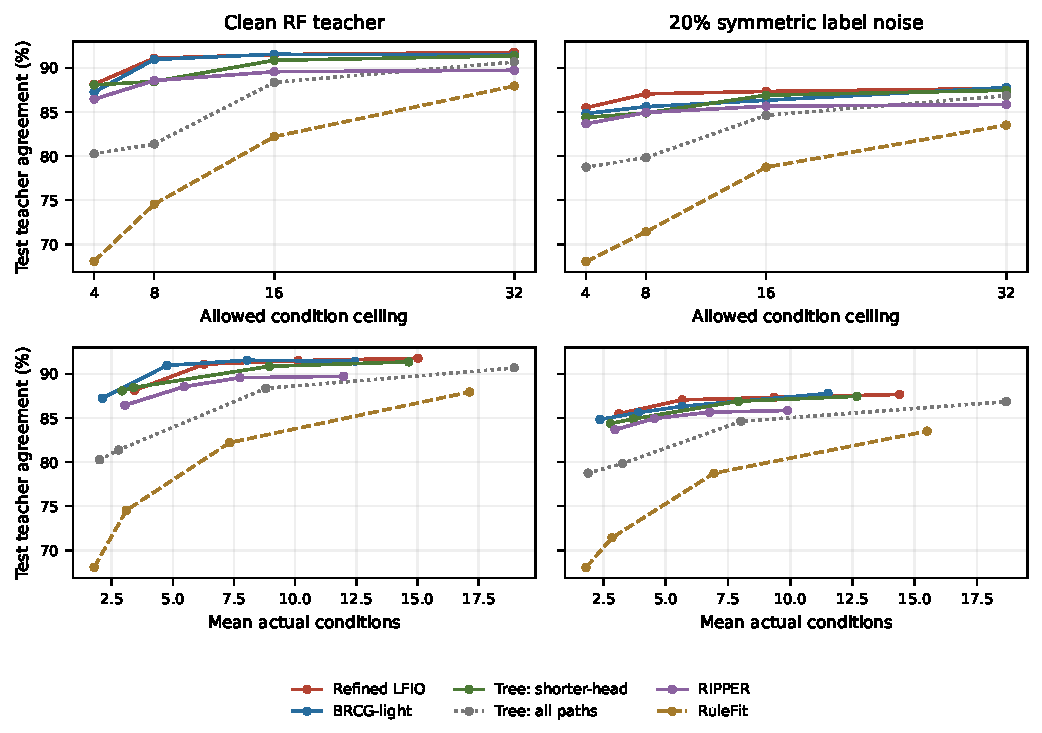
\includegraphics[width=\linewidth]{budget_frontier.pdf}
\caption{Validation-selected fidelity in the initial ten-dataset extension. The upper panels show allowed condition ceilings; the lower panels show actual mean conditions of the same selected models. Both tree encodings are displayed. Each noise level contains 50 paired settings. At four conditions, RuleFit is feasible on \RuleFitFourFeasibleClean/50 clean and \RuleFitFourFeasibleNoisy/50 noisy settings; every other displayed point uses all 50. Lines join the four prespecified budget selections; they are neither test-selected optima nor certified Pareto frontiers.}
\label{fig:budget}
\end{kbfigure}
At the primary eight-condition endpoint, Refined LFIO obtains \NewRefinedClean\% fidelity for clean random-forest teachers and \NewRefinedNoisy\% with symmetric observed-label noise. BRCG-light obtains \NewBRCGClean\% and \NewBRCGNoisy\%; RIPPER obtains \NewRipperClean\% and \NewRipperNoisy\%. Table~\ref{tab:strength_paired} reports the matched-setting differences and intervals, while Appendix~\ref{app:extension} retains all ten datasets and feasibility counts. All methods, including the expanded neural grids, are feasible on all 50 settings per condition at this endpoint.

On the same 50 settings per condition, teacher balanced accuracy against unchanged reference labels is \NewTeacherBAClean\% clean and \NewTeacherBANoisy\% noisy. The eight-condition Refined LFIO surrogates attain \NewRefinedBAClean\% and \NewRefinedBANoisy\%, respectively. These reference-label measurements distinguish successful teacher approximation from correct classification.

The clean-teacher difference from BRCG-light is 0.14 percentage points (descriptive 95\% interval [-1.12, 1.78]), which does not establish a clear advantage. Under symmetric noise the difference is 1.45 percentage points (descriptive 95\% interval [0.29, 2.76]). The corresponding differences from RIPPER are 2.54 percentage points (descriptive 95\% interval [0.47, 5.62]) for clean teachers and 2.12 percentage points (descriptive 95\% interval [0.47, 4.26]) under noise. Thus the evidence is stronger for the specified noisy-teacher setting than for clean-teacher superiority over a direct Boolean optimizer.

The expanded neural grids address the earlier small-budget feasibility problem. TT-Sparse is feasible on 50/50 clean-teacher settings, with 87.34\% mean fidelity and 50/50 noisy-teacher settings, with 84.30\% mean fidelity. NeuRules is feasible on 50/50 clean-teacher settings, with 86.76\% mean fidelity and 50/50 noisy-teacher settings, with 83.98\% mean fidelity. These are selected small-program results under the shared Boolean vocabulary, distinct from each method's native benchmark setting.

An exploratory restriction to the four newly added datasets gives Refined LFIO minus BRCG-light differences of 0.11 percentage points (descriptive 95\% interval [-1.54, 1.94]) for clean teachers and 0.62 percentage points (descriptive 95\% interval [-0.46, 2.38]) under noise. Both intervals include zero. The broader ten-dataset finding therefore provides stronger evidence than this four-dataset subset alone.


At the dataset level, the clean-teacher Refined-minus-BRCG comparison yields two wins, three ties, and five losses; the noisy comparison yields seven wins, two ties, and one loss. These counts use five-seed dataset means. A small positive aggregate clean difference therefore does not mean that most datasets improve. Actual mean conditions are 6.28/5.66 for Refined LFIO and 4.76/3.90 for BRCG-light: a shared ceiling does not imply identical deployed size.

\begin{kbtable}
\centering
\caption{Retrospective teacher-quality diagnostics for the original main cohort. BA uses unchanged reference labels; constant fidelity uses the majority teacher class chosen on validation. One-class counts refer to test teacher predictions. High fidelity to an uninformative teacher need not imply useful classification.}
\label{tab:teacher_quality}
\small
\begin{adjustbox}{max width=\linewidth}
\begin{tabular}{lrrrrrr}
\toprule
Dataset & Clean teacher BA & Clean constant fid. & Clean 1-class & Noisy teacher BA & Noisy constant fid. & Noisy 1-class \\
\midrule
Breast cancer & 94.50 & 62.98 & 0/5 & 87.46 & 61.23 & 0/5 \\
Banknote & 87.75 & 52.00 & 0/5 & 87.66 & 52.07 & 0/5 \\
Ionosphere & 79.36 & 72.16 & 0/5 & 73.73 & 64.19 & 0/5 \\
Spambase & 94.11 & 60.50 & 0/5 & 88.38 & 61.00 & 0/5 \\
Red wine & 69.06 & 53.38 & 0/5 & 64.09 & 53.31 & 0/5 \\
Grid simulation & 70.23 & 65.56 & 0/5 & 65.57 & 61.89 & 0/5 \\
MAGIC simulation & 72.08 & 76.70 & 0/5 & 71.04 & 75.43 & 0/5 \\
Haberman & 53.82 & 86.89 & 0/5 & 51.74 & 81.31 & 2/5 \\
Sonar & 82.39 & 58.57 & 0/5 & 72.86 & 57.14 & 0/5 \\
Transfusion & 54.69 & 94.10 & 0/5 & 53.99 & 95.31 & 1/5 \\
\bottomrule
\end{tabular}
\end{adjustbox}
\end{kbtable}

The constant reference obtains 68.28\% clean and 66.29\% noisy fidelity across the ten datasets. Refined LFIO's advantage over this diagnostic shows that the aggregate result is not solely explained by constant prediction. Individual near-perfect scores still require context: Haberman and transfusion each reduce to eight Boolean input patterns, all present in fitting and test partitions, while their clean teachers achieve only 53.82\% and 54.69\% reference-label balanced accuracy. Banknote has 15 fitting patterns in every original seed and 15--16 patterns over the full dataset, with 12--14 in test; its near-perfect fidelity is consequently a weak test of rich-boundary extraction. These are task-complexity limitations despite raw-duplicate grouping. Three noisy test teachers predict only one class; the balanced-fidelity diagnostic excludes these settings and reports that denominator explicitly.


\subsection{Components at the same condition ceiling}
\begin{kbtable}
\centering
\caption{Matched-budget 2-by-2 component ablation: teacher fidelity (percent) over 50 paired settings per noise level. All four configurations reselect the same depth, head, and penalty grids under the displayed hard ceiling.}
\label{tab:strength_ablation}
\small
\begin{adjustbox}{max width=\linewidth}
\begin{tabular}{lrrrrr}
\toprule
Components & Teacher & $B=4$ & $B=8$ & $B=16$ & $B=32$ \\
\midrule
Refined LFIO & Clean & 88.14 & 91.10 & 91.51 & 91.77 \\
Refined LFIO & Noisy & 85.48 & 87.05 & 87.33 & 87.67 \\
No pure start & Clean & 88.15 & 90.74 & 91.06 & 91.26 \\
No pure start & Noisy & 85.48 & 86.87 & 87.34 & 87.48 \\
No repair & Clean & 87.94 & 90.18 & 90.58 & 90.46 \\
No repair & Noisy & 85.31 & 86.96 & 87.40 & 87.53 \\
Neither component & Clean & 87.94 & 90.07 & 90.31 & 90.35 \\
Neither component & Noisy & 85.31 & 86.71 & 87.15 & 87.28 \\
\bottomrule
\end{tabular}
\end{adjustbox}
\end{kbtable}

The factorial comparison keeps the condition ceiling fixed; actual selected sizes can still differ. Because validation can choose either initial or repaired programs, enabling repair expands the considered programs without forcing deployment of a changed program. It can nevertheless reduce test fidelity through validation selection error. Component effects, including intervals at eight conditions, are therefore reported as empirical properties of this collection rather than universal gains.
At eight conditions, adding repair to the two-start learner changes clean-teacher fidelity by 0.92 percentage points (descriptive 95\% interval [0.13, 1.88]). The noisy-teacher change is only 0.09 percentage points (descriptive 95\% interval [-0.27, 0.55]). Adding the pure start when repair is already enabled changes clean and noisy fidelity by 0.36 percentage points (descriptive 95\% interval [-0.21, 1.06]) and 0.18 percentage points (descriptive 95\% interval [-0.23, 0.79]), respectively. These results support a clean-teacher repair benefit in this collection, while the pure-start and noisy repair effects remain inconclusive. The full method is never worse on the saved validation balanced-accuracy criterion than any component restriction; the same ordering need not hold on held-out fidelity.
The neither-component restriction already achieves 86.71\% noisy-teacher fidelity. Much of the full method's noisy advantage over BRCG-light is therefore shared with ordinary greedy construction, rather than isolated as an effect of the two added components.


The complete four-budget grid takes a median 8.35 seconds for the full method, versus 0.61 seconds with both components disabled and 2.79 seconds without the pure start. These approximately 13.7-fold and threefold cost differences are descriptive under parallel load. They motivate checking whether the component effects persist when the additional programs do not receive additional validation opportunities.

\subsection{Equal validation opportunities}\label{sec:slots}
\begin{kbtable}
\centering
\caption{Equal-validation-opportunity follow-up at eight conditions: ten datasets, five fresh split seeds, 50 settings per noise level. One/cell admits only the lowest-training-objective program from each depth/penalty/head cell. The four controls have identical slot counts within every setting; counts need not represent unique predictions. The original validation policy is the unchanged proposed method. Fidelity is percent; actual conditions and mean slots are shown.}
\label{tab:followup_slots}
\small
\begin{adjustbox}{max width=\linewidth}
\begin{tabular}{lrrrrrr}
\toprule
Configuration & Clean fidelity & Clean cond. & Clean slots & Noisy fidelity & Noisy cond. & Noisy slots \\
\midrule
Original validation policy & 90.87 & 5.92 & 78.16 & 86.62 & 5.78 & 77.94 \\
One/cell: both + repair & 91.03 & 5.64 & 28.00 & 86.60 & 5.72 & 28.00 \\
One/cell: ordinary + repair & 90.90 & 5.38 & 28.00 & 86.92 & 5.78 & 28.00 \\
One/cell: both, no repair & 90.35 & 5.44 & 28.00 & 86.20 & 5.30 & 28.00 \\
One/cell: ordinary, no repair & 90.03 & 5.22 & 28.00 & 86.20 & 5.30 & 28.00 \\
\bottomrule
\end{tabular}
\end{adjustbox}
\end{kbtable}

\begin{kbtable}
\centering
\caption{Paired ordinary-fidelity differences for the validation-slot controls. Eight conditions is this follow-up's primary endpoint; 16 is secondary. Each contrast has 50 paired settings per noise level. Intervals are descriptive hierarchical bootstrap intervals.}
\label{tab:followup_slot_differences}
\small
\begin{adjustbox}{max width=\linewidth}
\begin{tabular}{lrrr}
\toprule
Contrast & Budget & Clean $\Delta$ (pp), 95\% interval & Noisy $\Delta$ (pp), 95\% interval \\
\midrule
Repair with both starts & 8 & 0.68 [-0.40, 1.95] & 0.40 [-0.19, 1.13] \\
Pure start with repair & 8 & 0.13 [-0.98, 1.07] & -0.32 [-1.40, 0.13] \\
Both components & 8 & 1.00 [-0.23, 2.34] & 0.40 [-0.19, 1.13] \\
Original minus one/cell policy & 8 & -0.16 [-0.46, 0.01] & 0.03 [-0.08, 0.13] \\
Repair with both starts & 16 & 1.19 [0.08, 2.60] & 0.48 [-0.42, 1.44] \\
Pure start with repair & 16 & 0.65 [-0.01, 1.56] & 0.00 [-1.34, 1.16] \\
Both components & 16 & 1.51 [0.34, 2.90] & 0.48 [-0.42, 1.44] \\
Original minus one/cell policy & 16 & -0.73 [-1.71, -0.02] & 0.20 [-0.20, 0.77] \\
\bottomrule
\end{tabular}
\end{adjustbox}
\end{kbtable}

With one validation candidate per grid cell, adding repair to both starts changes ordinary fidelity by 0.68 [-0.40, 1.95] percentage points for clean teachers and 0.40 [-0.19, 1.13] under noise (descriptive 95\% intervals in brackets). Both intervals include zero. Adding the pure start with repair gives 0.13 [-0.98, 1.07] and -0.32 [-1.40, 0.13] percentage points, respectively. Thus the positive mean repair effects are not stable enough in this follow-up to establish a clear advantage after controlling validation opportunities; the pure-start effect remains inconclusive. The original validation policy versus the one-per-cell full control differs by -0.16 [-0.46, 0.01] and 0.03 [-0.08, 0.13] percentage points. These controls leave training search and computational effort unequal. They do not redefine the deployed method or establish equivalence.

At the prespecified secondary sixteen-condition ceiling, the same repair contrast is 1.19 [0.08, 2.60] percentage points for clean teachers and 0.48 [-0.42, 1.44] under noise. The clean interval excludes zero, giving narrower evidence for repair at this larger ceiling; the noisy and pure-start effects remain inconclusive. This secondary result does not replace the eight-condition endpoint.


\subsection{Repair versus restarts at equal scored work}\label{sec:work-results}
\begin{kbtable}
\centering
\caption{Scored-work allocation at eight conditions: ten datasets, three new seeds and 30 settings per noise level. Each paired policy scores exactly $m$ times the supported pool size per grid cell and submits one fitting-objective winner to validation. Scores and CPU are medians over all 60 settings; CPU excludes shared candidate preparation. Matching score counts does not match wall time or instructions.}
\label{tab:checklist_work}
\small
\begin{adjustbox}{max width=\linewidth}
\begin{tabular}{lrrrrrr}
\toprule
Policy & $m$ & Clean fidelity & Noisy fidelity & Conditions C/N & Scores (M) & CPU (s) \\
\midrule
Greedy restarts & 8 & 90.84 & 87.27 & 5.83/5.73 & 0.444 & 0.26 \\
Repair allocation & 8 & 90.93 & 87.40 & 5.53/5.50 & 0.444 & 0.32 \\
Greedy restarts & 32 & 91.03 & 87.14 & 6.17/5.60 & 1.776 & 0.99 \\
Repair allocation & 32 & 90.92 & 87.44 & 5.73/5.83 & 1.776 & 1.27 \\
\bottomrule
\end{tabular}
\end{adjustbox}
\end{kbtable}

\begin{kbtable}
\centering
\caption{Four contrasts fixed before the new fits, all at eight conditions. Paired hierarchical bootstrap intervals are descriptive. The 98.75\% individual intervals provide a Bonferroni-style sensitivity for four comparisons; they do not validate population sampling or remove dependence from reused observations.}
\label{tab:checklist_primary}
\small
\begin{adjustbox}{max width=\linewidth}
\begin{tabular}{lrrrr}
\toprule
Primary contrast & Teacher & $\Delta$ (pp), 95\% & $\Delta$ (pp), 98.75\% & Pairs \\
\midrule
Repair minus restarts, $m=32$ & Clean & -0.10 [-1.14, 1.04] & -0.10 [-1.42, 1.43] & 30 \\
Repair minus restarts, $m=32$ & Noisy & 0.30 [-0.31, 1.47] & 0.30 [-0.40, 1.88] & 30 \\
MDL minus quantile, Refined & Clean & 0.07 [-2.06, 2.49] & 0.07 [-2.47, 3.23] & 30 \\
MDL minus quantile, Refined & Noisy & -0.70 [-3.94, 2.96] & -0.70 [-5.00, 4.48] & 30 \\
\bottomrule
\end{tabular}
\end{adjustbox}
\end{kbtable}

At the primary allowance $m=32$, allocating scores to repair rather than additional greedy restarts changes fidelity by -0.10 [-1.14, 1.04] percentage points for clean teachers and 0.30 [-0.31, 1.47] under noise. The corresponding 98.75\% sensitivity intervals are -0.10 [-1.42, 1.43] and 0.30 [-0.40, 1.88]. Table~\ref{tab:checklist_work} reports actual score counts and CPU costs, and Table~\ref{tab:checklist_secondary} retains the lower-allowance comparison. These are bounded search policies with one validation winner per cell; they do not retrospectively change the original Refined LFIO algorithm or its results.

All four latest primary 95\% intervals include zero, as do their wider multiplicity-sensitivity intervals. This does not establish equivalence. The scored-work experiment specifically fails to show that allocating the fixed allowance to local repair generalizes better than using it for additional randomized greedy starts. Its median CPU cost is 1.27 versus 0.99 seconds at $m=32$, illustrating why identical objective-score counts should not be described as identical computational time.


\subsection{Teacher, noise, and representation sensitivity}
\begin{kbtable}
\centering
\caption{Eight-condition sensitivity on ten datasets and three seeds. Method columns report teacher fidelity (percent) and feasible settings out of 30; final columns report balanced accuracy against unchanged test reference labels. HGB is histogram gradient boosting. Native RF sees continuous inputs; every surrogate still sees Boolean inputs.}
\label{tab:strength_sensitivity}
\small
\begin{adjustbox}{max width=\linewidth}
\begin{tabular}{lrrrrrr}
\toprule
Scenario & Refined LFIO & BRCG-light & RIPPER & Tree & Teacher BA & Refined BA \\
\midrule
RF, clean & 90.70 (30) & 90.61 (30) & 88.09 (30) & 80.57 (30) & 74.87 & 72.92 \\
RF, symmetric 20\% & 86.38 (30) & 85.24 (30) & 84.73 (30) & 79.70 (30) & 71.12 & 71.12 \\
RF, asymmetric & 85.96 (30) & 85.99 (30) & 83.74 (30) & 83.80 (30) & 67.36 & 70.09 \\
RF, feature-dependent & 86.33 (30) & 85.67 (30) & 83.82 (30) & 77.55 (30) & 71.04 & 73.22 \\
HGB, clean & 93.33 (30) & 92.81 (30) & 90.19 (30) & 81.33 (30) & 74.84 & 73.32 \\
HGB, symmetric 20\% & 91.10 (30) & 89.28 (30) & 86.77 (30) & 80.84 (30) & 72.51 & 71.95 \\
Logistic, clean & 92.31 (30) & 92.81 (30) & 89.37 (30) & 82.98 (30) & 74.71 & 72.94 \\
Logistic, symmetric 20\% & 90.82 (30) & 90.42 (30) & 88.80 (30) & 83.14 (30) & 72.40 & 71.61 \\
Native RF, clean & 80.04 (30) & 81.64 (30) & 78.20 (30) & 75.41 (30) & 83.07 & 75.82 \\
Native RF, symmetric 20\% & 73.78 (30) & 76.08 (30) & 73.27 (30) & 72.35 (30) & 78.34 & 72.95 \\
\bottomrule
\end{tabular}
\end{adjustbox}
\end{kbtable}

\begin{kbtable}
\centering
\caption{Complexity-counting sensitivity: fidelity after validation reselection under each convention. The alternative tree export uses a shorter-head DNF and opposite default, with exact prediction agreement. All displayed methods are feasible on all 50 settings. Other model counts are unchanged.}
\label{tab:strength_counting}
\small
\begin{adjustbox}{max width=\linewidth}
\begin{tabular}{lrrrr}
\toprule
Teacher & Budget & Refined LFIO & Tree leaf paths & Tree single-head DNF \\
\midrule
Clean & 4 & 88.14 & 80.25 & 88.07 \\
Clean & 8 & 91.10 & 81.36 & 88.46 \\
Clean & 16 & 91.51 & 88.36 & 90.86 \\
Clean & 32 & 91.77 & 90.69 & 91.36 \\
Noisy & 4 & 85.48 & 78.75 & 84.37 \\
Noisy & 8 & 87.05 & 79.83 & 84.89 \\
Noisy & 16 & 87.33 & 84.62 & 86.90 \\
Noisy & 32 & 87.67 & 86.86 & 87.46 \\
\bottomrule
\end{tabular}
\end{adjustbox}
\end{kbtable}

The additional scenarios separate three sources of variation: changed teacher functions, changed corruption mechanisms, and information unavailable to the Boolean student. Fidelity and reference-label balanced accuracy answer different questions. In particular, high agreement with a nearly constant or inaccurate teacher is weak evidence for an informative explanation. Saved teacher predictions, realized noise rates, per-dataset metrics, and feature diagnostics allow these cases to be identified.
With three paired seeds, moving the RF teacher from Boolean to native numerical inputs changes Refined LFIO fidelity from 90.70\% to 80.04\% for clean teachers and from 86.38\% to 73.78\% under symmetric noise. BRCG-light reaches 81.64\% and 76.08\% in those native-teacher settings. This reversal qualifies any broad superiority claim and shows the difficulty of approximating native-input teachers with the present vocabulary and search.

At eight conditions over all five main splits, the equivalent shorter-head tree export raises clean/noisy tree fidelity from 81.36\%/79.83\% to 88.46\%/84.89\%. The smaller difference under equivalent tree encoding demonstrates that part of the original tree gap was due to complexity accounting.


\subsection{Native numerical teachers and richer predicates}\label{sec:native-followup}
\begin{kbtable}
\centering
\caption{Native-input RF teachers: ten datasets and three fresh split seeds, eight-condition ceiling. Refined LFIO and BRCG-light both use maximum conjunction depth two in both vocabulary arms. Thresholds are fit-only median or quartiles plus median; BRCG-light searches 30 penalty/polarity configurations. The shorter-head tree uses supervised native thresholds. Fidelity is percent; conditions are actual sizes.}
\label{tab:followup_native}
\small
\begin{adjustbox}{max width=\linewidth}
\begin{tabular}{lrrrrrr}
\toprule
Student & Clean fidelity & Clean cond. & Clean feasible & Noisy fidelity & Noisy cond. & Noisy feasible \\
\midrule
Refined, median & 79.80 & 4.77 & 30/30 & 75.77 & 4.37 & 30/30 \\
Refined, three quantiles & 83.19 & 6.23 & 30/30 & 79.06 & 6.50 & 30/30 \\
BRCG-light, median & 81.79 & 4.93 & 30/30 & 77.15 & 3.30 & 30/30 \\
BRCG-light, three quantiles & 84.11 & 5.40 & 30/30 & 79.91 & 4.07 & 30/30 \\
Tree, native thresholds & 82.54 & 3.27 & 30/30 & 77.88 & 2.87 & 30/30 \\
\bottomrule
\end{tabular}
\end{adjustbox}
\end{kbtable}

\begin{kbtable}
\centering
\caption{Paired native-teacher comparisons at eight conditions, using only shared feasible settings. The vocabulary effects use the same fixed depth and selection grids within each method; the tree learns its own thresholds.}
\label{tab:followup_native_differences}
\small
\begin{adjustbox}{max width=\linewidth}
\begin{tabular}{lrrrr}
\toprule
Contrast & Clean $\Delta$ (pp), 95\% interval & Clean pairs & Noisy $\Delta$ (pp), 95\% interval & Noisy pairs \\
\midrule
Refined: three quantiles minus median & 3.40 [0.12, 6.52] & 30 & 3.30 [0.76, 6.20] & 30 \\
BRCG: three quantiles minus median & 2.32 [0.81, 3.91] & 30 & 2.75 [0.91, 4.85] & 30 \\
Refined minus BRCG, three quantiles & -0.92 [-4.25, 2.11] & 30 & -0.84 [-4.82, 2.18] & 30 \\
Refined three quantiles minus native tree & 0.65 [-3.03, 4.03] & 30 & 1.18 [-3.18, 5.05] & 30 \\
\bottomrule
\end{tabular}
\end{adjustbox}
\end{kbtable}

With native-input teachers, replacing the median vocabulary by three fit-only quantiles raises Refined LFIO's mean fidelity from 79.80\% to 83.19\% for clean teachers and from 75.77\% to 79.06\% under noise. The paired changes are 3.40 [0.12, 6.52] and 3.30 [0.76, 6.20] percentage points. BRCG-light also improves with the richer vocabulary, reaching 84.11\% and 79.91\%. Refined LFIO minus BRCG-light under the shared three-quantile vocabulary is -0.92 [-4.25, 2.11] and -0.84 [-4.82, 2.18] percentage points; both intervals include zero. The stronger evidence therefore concerns the numerical predicate vocabulary, rather than superiority over the direct Boolean comparator. The richer vocabulary increases the available candidate pool and often the selected size, so it does not isolate representation from all search-cost effects. Median complete-grid wall time for Refined LFIO rises from 0.53 to 7.03 seconds; BRCG-light rises from 7.53 to 23.60 seconds. These timings describe the four-budget grids under parallel load.


\subsection{Quantifying vocabulary information loss}\label{sec:ceiling-results}
\begin{kbtable}
\centering
\caption{Retrospective empirical vocabulary ceilings on frozen native-teacher test sets. Entries are clean/noisy percentages, except predicate counts. Each cohort contains ten datasets and three seeds per noise level; means weight datasets equally. Refined LFIO fidelity uses the unchanged eight-condition selections. The median in the later cohort is an encoding diagnostic only, with no fitted student. Distance to the unrestricted decoder ceiling also includes capacity, fitting and selection effects; it is not a certified optimization gap.}
\label{tab:vocabulary_ceiling}
\small
\begin{adjustbox}{max width=\linewidth}
\begin{tabular}{llrrrr}
\toprule
Split seeds & Vocabulary & Predicates & Ceiling & Refined fidelity & Distance (pp) \\
\midrule
4001--4003 & Median & 22.50/22.50 & 92.75/91.08 & 79.80/75.77 & 12.96/15.32 \\
4001--4003 & Quantile & 57.80/57.80 & 98.26/97.43 & 83.19/79.06 & 15.07/18.37 \\
5001--5003 & Median & 22.50/22.50 & 92.90/90.74 & --/-- & --/-- \\
5001--5003 & Quantile & 57.80/57.80 & 98.17/97.23 & 85.68/80.29 & 12.49/16.94 \\
5001--5003 & MDL & 46.70/37.23 & 95.72/93.86 & 85.75/79.59 & 9.97/14.27 \\
\bottomrule
\end{tabular}
\end{adjustbox}
\end{kbtable}

On seeds 4001--4003, median encodings limit the dataset-equal empirical test fidelity to 92.75\% clean and 91.08\% noisy. Three fitting-only quantiles raise these ceilings to 98.26\% and 97.43\%, respectively. Thus a measurable part of the disagreement is already unavoidable before rule search. The selected students remain below both ceilings, leaving additional capacity and fitting limitations.

On the separate seeds 5001--5003, quantile ceilings are 98.17\%/97.23\% clean/noisy; the smaller MDL vocabularies give 95.72\%/93.86\%. MDL therefore does not retain all distinctions available to the quantile decoder, despite similar aggregate fidelity of the selected small programs. The two vocabularies are not nested, so no monotonicity theorem orders them. Both retain the median and satisfy its refinement bound in every audited partition.

These quantities clarify what the richer predicates change. They separate an empirical obstruction shared by all deterministic students from the fidelity reached by a particular fitted rule program. They do not attribute the entire observed gain to reduced collisions: the candidate pool, selected size, and fitting cost also change. The ceiling is 100\% in some high-dimensional settings, where absence of collisions on the finite test sample provides no evidence of adequate population representation. Per-dataset results, singleton counts, and fitting/validation ceilings accompany the aggregate table.

\subsection{Fitting-teacher-informed predicates}\label{sec:mdl-results}
\begin{kbtable}
\centering
\caption{Native-teacher follow-up at eight conditions. Both vocabularies allow at most three predicates per original feature; actual vocabulary sizes differ. Median plus MDL uses only fitting teacher labels. All arms use the prespecified selection grids. Parentheses report feasibility. Median wall time covers all four condition budgets, includes preprocessing (and LFIO candidate preparation), and is affected by parallel load.}
\label{tab:checklist_vocabulary}
\small
\begin{adjustbox}{max width=\linewidth}
\begin{tabular}{lrrrrr}
\toprule
Method & Clean fidelity & Noisy fidelity & Conditions C/N & Predicates C/N & Wall (s) \\
\midrule
Refined, quantiles & 85.68 (30/30) & 80.29 (30/30) & 6.63/6.00 & 57.8/57.8 & 8.45 \\
Refined, median + MDL & 85.75 (30/30) & 79.59 (30/30) & 5.67/5.80 & 46.7/37.2 & 3.63 \\
BRCG, quantiles & 85.85 (30/30) & 80.33 (30/30) & 5.23/4.33 & 57.8/57.8 & 22.39 \\
BRCG, median + MDL & 86.33 (30/30) & 80.81 (30/30) & 4.50/3.57 & 46.7/37.2 & 19.20 \\
Native tree & 84.94 (30/30) & 80.44 (30/30) & 3.03/3.57 & -- & 0.06 \\
\bottomrule
\end{tabular}
\end{adjustbox}
\end{kbtable}

\begin{kbtable}
\centering
\caption{Secondary paired contrasts in the new three-seed cohort. Intervals are unadjusted descriptive 95\% intervals. These do not establish a universal method ranking or replace the four fixed primary contrasts.}
\label{tab:checklist_secondary}
\small
\begin{adjustbox}{max width=\linewidth}
\begin{tabular}{lrrr}
\toprule
Secondary contrast & Teacher & $\Delta$ (pp), 95\% & Pairs \\
\midrule
Repair minus restarts, $m=8$ & Clean & 0.08 [-0.53, 0.77] & 30 \\
Repair minus restarts, $m=8$ & Noisy & 0.13 [-0.45, 0.75] & 30 \\
BRCG: MDL minus quantile & Clean & 0.49 [-2.30, 3.76] & 30 \\
MDL: Refined minus BRCG & Clean & -0.58 [-2.66, 1.23] & 30 \\
MDL Refined minus native tree & Clean & 0.80 [-2.94, 3.98] & 30 \\
BRCG: MDL minus quantile & Noisy & 0.49 [-1.66, 2.57] & 30 \\
MDL: Refined minus BRCG & Noisy & -1.22 [-5.35, 2.39] & 30 \\
MDL Refined minus native tree & Noisy & -0.85 [-5.56, 2.75] & 30 \\
\bottomrule
\end{tabular}
\end{adjustbox}
\end{kbtable}

Replacing fixed quantiles by median plus fitting-teacher MDL cuts changes Refined LFIO fidelity by 0.07 [-2.06, 2.49] percentage points clean and -0.70 [-3.94, 2.96] under noise. The 98.75\% sensitivity intervals are 0.07 [-2.47, 3.23] and -0.70 [-5.00, 4.48]. Both vocabularies have the same maximum of three predicates per feature, but the MDL arm can retain fewer. Its effect therefore combines cut placement, supervised selection, and actual vocabulary size; it is not evidence for a new discretization principle.

The numerical means for median-plus-MDL versus fixed quantiles are 85.75\% versus 85.68\% clean and 79.59\% versus 80.29\% noisy. Median full-grid wall time falls from 8.45 to 3.63 seconds for Refined LFIO and from 22.39 to 19.20 seconds for BRCG-light. These costs include preprocessing and are descriptive under parallel load. Smaller actual vocabularies and programs are a useful engineering tradeoff, but the uncertainty does not prove preservation of fidelity. Comparisons against BRCG-light and the native tree also remain inconclusive. We retain both fixed and adaptive vocabularies as explicit options, with no test-selected change of default.

\subsection{Concrete repair trajectories}\label{sec:cases}
Table~\ref{tab:repair_cases} contrasts two replayed repairs and their held-out consequences.
\begin{kbtable}
\centering
\caption{Two post-hoc illustrations from the new eight-condition cohort: one positive and one negative held-out repair change, preferring breast-cancer features and then larger normalized training gain. The exported programs match saved selected models. Thresholds are shown to seven significant digits; full precision is retained in the supplement. Ionosphere feature indices are zero based. These examples are not independent validation.}
\label{tab:repair_cases}
\small
\begin{tabular}{llrrrr}
\toprule
Case & Stage & Training $J$ & Conditions & Validation BA (\%) & Test fidelity (\%) \\
\midrule
A & Before & 66.48 & 8 & 88.05 & 86.84 \\
A & After & 65.27 & 8 & 93.44 & 87.72 \\
B & Before & 63.63 & 2 & 60.00 & 84.29 \\
B & After & 28.07 & 8 & 85.00 & 80.00 \\
\bottomrule
\end{tabular}
\par\medskip
\begin{minipage}[t]{0.48\linewidth}\raggedright\small
\textbf{Case A: Breast cancer, seed 4002, noisy teacher.}\par\smallskip
\textbf{Before.} Head 1, default 0.\par Rule 1: mean radius \(> 13.4\) \textbf{and} mean concavity \(> 0.06181\) \textbf{and} mean concave points \(> 0.0339\).\par Rule 2: mean radius \(> 13.4\) \textbf{and} mean concave points \(\leq 0.0339\) \textbf{and} area error \(> 24.44\).\par Rule 3: mean perimeter \(> 86.1\) \textbf{and} worst radius \(\leq 14.8\).\par\smallskip
\textbf{After.} Head 1, default 0.\par Rule 1: mean radius \(> 13.4\) \textbf{and} mean concave points \(\leq 0.0339\) \textbf{and} area error \(> 24.44\).\par Rule 2: mean perimeter \(> 86.1\) \textbf{and} worst radius \(\leq 14.8\).\par Rule 3: mean concavity \(> 0.06181\) \textbf{and} worst area \(> 663.5\) \textbf{and} worst concave points \(> 0.09993\).\par\smallskip
\end{minipage}\hfill
\begin{minipage}[t]{0.48\linewidth}\raggedright\small
\textbf{Case B: Ionosphere, seed 4001, clean teacher.}\par\smallskip
\textbf{Before.} Head 0, default 1.\par Rule 1: x26 \(> 0.73886\) \textbf{and} x28 \(\leq 0.4764\).\par\smallskip
\textbf{After.} Head 0, default 1.\par Rule 1: x26 \(> 0.73886\) \textbf{and} x28 \(\leq 0.4764\).\par Rule 2: x9 \(\leq 0.01829\) \textbf{and} x16 \(\leq 0.58373\).\par Rule 3: x22 \(\leq 0.57528\) \textbf{and} x26 \(> 0.73886\).\par Rule 4: x11 \(\leq 0.0213\) \textbf{and} x20 \(\leq 0.50464\).\par\smallskip
\end{minipage}
\end{kbtable}
Case A uses replace. On fitting teacher targets, it corrects 2 false head predictions and 2 missed head predictions, while introducing 2 false head predictions and 1 missed head predictions. The training reduction accompanies better held-out fidelity.

Case B uses add, add, add, replace. On fitting teacher targets, it corrects 0 false head predictions and 36 missed head predictions, while introducing 14 false head predictions and 0 missed head predictions. The training reduction and validation selection do not prevent worse held-out fidelity.




\subsection{Computational cost and feature consistency}
\begin{kbtable}
\centering
\caption{Computation per dataset/seed/noise setting for the complete four-budget selection grid. LFIO wall time includes candidate preparation; the recorded CPU interval excludes preparation. Candidate counts are final budget fits for LFIO and external configurations otherwise; LFIO also searches an inner grid. Parallel execution on an AMD Threadripper PRO 5995WX makes wall times load dependent.}
\label{tab:strength_runtime}
\small
\begin{adjustbox}{max width=\linewidth}
\begin{tabular}{lrrrrr}
\toprule
Method & Median wall (s) & 90th pct. (s) & Median CPU (s) & Fitted candidates & Inner validation programs \\
\midrule
Refined LFIO & 8.35 & 60.82 & 8.26 & 4.00 & 272.00 \\
No pure start & 2.79 & 24.74 & 2.71 & 4.00 & 128.00 \\
No repair & 0.73 & 8.16 & 0.66 & 4.00 & 180.00 \\
Neither component & 0.61 & 7.70 & 0.54 & 4.00 & 96.00 \\
Tree & 0.05 & 0.22 & 0.05 & 12.00 & -- \\
RIPPER & 1.99 & 12.12 & 1.99 & 24.00 & -- \\
RuleFit & 5.56 & 10.33 & 5.55 & 5.00 & -- \\
BRCG-light & 14.14 & 29.29 & 16.52 & 10.00 & -- \\
TT-Sparse & 4.91 & 15.09 & 4.87 & 8.00 & -- \\
NeuRules & 56.45 & 878.34 & 56.30 & 12.00 & -- \\
\bottomrule
\end{tabular}
\end{adjustbox}
\end{kbtable}

\begin{kbtable}
\centering
\caption{Validation teacher feature-consistency diagnostic at eight conditions. Feature mass is the percentage of normalized permutation-disagreement importance on features used by the surrogate. Zero total disagreement is undefined. This is not FI-rules4XAI evaluation or evidence of internal or causal fidelity; larger feature sets can cover more mass.}
\label{tab:strength_features}
\small
\begin{adjustbox}{max width=\linewidth}
\begin{tabular}{lrrrrrr}
\toprule
Method & Clean feature mass & Clean used features & Clean defined & Noisy feature mass & Noisy used features & Noisy defined \\
\midrule
Refined LFIO & 63.03 & 5.64 & 50 & 57.47 & 5.08 & 47 \\
BRCG-light & 56.75 & 4.30 & 50 & 44.41 & 3.36 & 47 \\
Tree & 20.52 & 1.26 & 50 & 24.81 & 1.40 & 47 \\
RIPPER & 56.79 & 4.54 & 50 & 51.39 & 3.80 & 47 \\
RuleFit & 34.06 & 2.18 & 50 & 31.92 & 1.98 & 47 \\
TT-Sparse & 51.07 & 3.88 & 50 & 47.71 & 3.70 & 47 \\
NeuRules & 51.48 & 3.72 & 50 & 48.18 & 3.54 & 47 \\
\bottomrule
\end{tabular}
\end{adjustbox}
\end{kbtable}

The complete-grid timings quantify the effort required to obtain compact predictors. Cached enumeration avoids repeating the same training-only work across budgets, but local repair still scans many candidate replacements. Candidate visits, inner validation-program counts, and per-dataset times are exported alongside the aggregate timing table. They do not support an equal-computation comparison or a claim of large-scale scalability.

Teacher-feature mass is reported separately from fidelity. It measures coverage of a permutation-based diagnostic by the surrogate's feature set, without testing whether those features act in the same way. A model can obtain high prediction agreement with a different feature subset, and redundant predictors can exchange attribution mass. These observations delimit the explanatory claim in the sense emphasized by FI-rules4XAI~\citep{kozielski2025}; no experimental superiority over that method is asserted.
\kbsbarrier

\appendix
\section{Extension details and reproduction}\label{app:extension}
\begin{kbtable}
\centering
\caption{Dataset characteristics. Positive-label definitions and source hashes are fixed in the protocol. Identical raw input vectors are grouped before partitioning; MAGIC and grid stability are simulated data.}
\label{tab:strength_data}
\small
\begin{adjustbox}{max width=\linewidth}
\begin{tabular}{lrrrr}
\toprule
Dataset & Rows & Inputs & Unique raw inputs & Positive (\%) \\
\midrule
Breast cancer & 569 & 30 & 569 & 37.26 \\
Banknote & 1372 & 4 & 1348 & 44.46 \\
Ionosphere & 351 & 34 & 350 & 64.10 \\
Spambase & 4601 & 57 & 4207 & 39.40 \\
Red wine & 1599 & 11 & 1359 & 53.47 \\
Grid simulation & 10000 & 12 & 10000 & 36.20 \\
MAGIC simulation & 19020 & 10 & 18905 & 64.84 \\
Haberman & 306 & 3 & 283 & 26.47 \\
Sonar & 208 & 60 & 208 & 53.37 \\
Transfusion & 748 & 4 & 502 & 23.80 \\
\bottomrule
\end{tabular}
\end{adjustbox}
\end{kbtable}

\begin{kbtable}
\centering
\caption{Eight-condition per-dataset fidelity (percent); parentheses give feasible splits out of five. Missing configurations are not assigned constant predictions.}
\label{tab:strength_datasets}
\small
\begin{adjustbox}{max width=\linewidth}
\begin{tabular}{lrrrrrrrr}
\toprule
Dataset & Teacher & Refined LFIO & BRCG-light & Tree & RIPPER & RuleFit & TT-Sparse & NeuRules \\
\midrule
Breast cancer & Clean & 96.32 (5) & 96.67 (5) & 88.07 (5) & 94.39 (5) & 62.98 (5) & 91.40 (5) & 95.44 (5) \\
Breast cancer & Noisy & 91.23 (5) & 89.12 (5) & 83.51 (5) & 87.37 (5) & 61.23 (5) & 87.37 (5) & 90.00 (5) \\
Banknote & Clean & 100.00 (5) & 100.00 (5) & 91.64 (5) & 100.00 (5) & 91.64 (5) & 96.00 (5) & 98.33 (5) \\
Banknote & Noisy & 99.85 (5) & 99.85 (5) & 92.44 (5) & 99.85 (5) & 93.45 (5) & 97.38 (5) & 98.47 (5) \\
Ionosphere & Clean & 85.48 (5) & 87.76 (5) & 67.86 (5) & 82.92 (5) & 64.82 (5) & 81.52 (5) & 72.45 (5) \\
Ionosphere & Noisy & 79.85 (5) & 79.00 (5) & 66.77 (5) & 72.14 (5) & 44.38 (5) & 72.99 (5) & 68.74 (5) \\
Spambase & Clean & 90.99 (5) & 92.12 (5) & 83.02 (5) & 89.69 (5) & 60.50 (5) & 86.04 (5) & 85.52 (5) \\
Spambase & Noisy & 86.51 (5) & 85.75 (5) & 81.17 (5) & 84.67 (5) & 61.00 (5) & 80.76 (5) & 80.00 (5) \\
Red wine & Clean & 83.44 (5) & 78.69 (5) & 77.06 (5) & 82.69 (5) & 63.88 (5) & 80.00 (5) & 78.38 (5) \\
Red wine & Noisy & 75.88 (5) & 71.25 (5) & 71.06 (5) & 74.38 (5) & 65.00 (5) & 72.94 (5) & 71.75 (5) \\
Grid simulation & Clean & 82.07 (5) & 82.07 (5) & 70.23 (5) & 67.65 (5) & 65.56 (5) & 75.49 (5) & 71.67 (5) \\
Grid simulation & Noisy & 70.67 (5) & 67.00 (5) & 66.23 (5) & 67.39 (5) & 61.89 (5) & 68.68 (5) & 67.54 (5) \\
MAGIC simulation & Clean & 95.36 (5) & 95.59 (5) & 76.70 (5) & 95.16 (5) & 93.23 (5) & 90.11 (5) & 94.09 (5) \\
MAGIC simulation & Noisy & 92.99 (5) & 92.64 (5) & 75.43 (5) & 91.92 (5) & 79.48 (5) & 90.95 (5) & 91.05 (5) \\
Haberman & Clean & 100.00 (5) & 100.00 (5) & 91.15 (5) & 100.00 (5) & 100.00 (5) & 100.00 (5) & 100.00 (5) \\
Haberman & Noisy & 100.00 (5) & 100.00 (5) & 95.41 (5) & 100.00 (5) & 100.00 (5) & 100.00 (5) & 100.00 (5) \\
Sonar & Clean & 77.62 (5) & 76.67 (5) & 73.81 (5) & 73.33 (5) & 48.57 (5) & 72.86 (5) & 72.86 (5) \\
Sonar & Noisy & 73.81 (5) & 71.43 (5) & 70.95 (5) & 71.90 (5) & 52.38 (5) & 71.90 (5) & 73.33 (5) \\
Transfusion & Clean & 99.73 (5) & 100.00 (5) & 94.10 (5) & 99.73 (5) & 94.10 (5) & 100.00 (5) & 98.93 (5) \\
Transfusion & Noisy & 99.73 (5) & 100.00 (5) & 95.31 (5) & 99.73 (5) & 95.31 (5) & 100.00 (5) & 98.93 (5) \\
\bottomrule
\end{tabular}
\end{adjustbox}
\end{kbtable}

The initial frozen extension protocol is \path{docs/research/STRENGTHENING_PROTOCOL_2026-09-21.md}. Execution uses \path{run_strengthening_experiments.py}; source/data hashes and package versions precede fitting in its manifest. The audit generator, \path{generate_strengthened_manuscript.py}, verifies source hashes, group separation, median fitting, validation selection, saved prediction metrics, and LFIO/BRCG/tree symbolic exports. Neural exports are checked against their native models during execution. The two counting conventions share fitted candidates and test predictions. The follow-up protocol is \path{docs/research/FOLLOWUP_PROTOCOL_2026-09-22.md}; execution and independent prediction audits use \path{run_review_followup.py} and \path{generate_review_revision.py}. Its 100 mechanism and 60 numerical-teacher settings produce 2,200 budget selections across 800 method grids. All selections retain fitting-only preprocessing and validation-only selection. New seeds reuse dataset observations and do not provide independent external data. Successful and unsuccessful rule examples are explicitly selected post hoc and exactly replayed from recorded configurations.

The initial extension comprises 340 teacher settings, 1,960 method grids including the 100-setting neural comparison, and 7,840 budget selections per counting convention. The latest protocol is \path{docs/research/SEARCH_VOCABULARY_PROTOCOL_2026-09-24.md}; \path{run_checklist_experiments.py} executes 120 additional settings, 540 method grids and 1,440 selections. \path{generate_checklist_revision.py} rebuilds fitting-only thresholds, checks paired per-cell score counts and validation choices, and reconstructs 5,040 candidate exports. These settings are not independent trials. Full metrics, warnings, timing, component differences, and teacher-feature diagnostics remain in the supplement. BRCG-light's Apache-licensed source is vendored with its commit and file hashes. \path{docs/research/REPRODUCE.md} gives commands and separates all cohorts.

Two execution amendments concern three single-class teacher settings. RuleFit's logistic solver rejects the fitting targets; an explicit adapter emits their exact constant program. TT-Sparse's validation AUC is undefined, so its pruning log stores null instead of a non-JSON NaN. The latter changes only serialization: the saved predictions before and after the amendment agree exactly, and training and pruning are unchanged. Original errors and separate adapter hashes are retained. Failed attempts are excluded from timing; no test score determines either amendment.
\kbsbarrier

\section{Earlier development and external evidence}\label{app:development}
Earlier exploratory work used breast cancer, banknote, ionosphere, and spambase with ten stratified 60/20/20 splits (seeds 1001--1010), fit-only median binarization, random-forest teachers, and symmetric noise 0/0.1/0.2. A later external check added red wine and simulated grid stability, grouped raw duplicates, and seeds 2001--2010. These studies informed the initial ten-dataset extension. Their unconstrained, direct-label, stability, and external-check tables remain in the accompanying machine-readable evidence; they are not pooled with either later cohort. The numerical records and original executable versions are retained. The paper presents only Refined LFIO as the named proposed method and uses component switches as controls.
\kbsbarrier

\section{Generated tasks and capacity controls}\label{app:synthetic}
The Sudoku input consists of row, column, and box non-duplication predicates. Queens uses row, column, diagonal, and count predicates. High scores indicate recovery from those supplied constraints, not discovery of spatial rules from raw boards. These older generated fitting experiments remain separate supplementary diagnostics.

To distinguish capacity from fitting, let $s(x)=\sum_{j=1}^5x_j$ and $h_k(x)=\mathbf{1}[s(x)>k-1/2]$. Then
\begin{equation}
 \operatorname{parity}(x)=\sum_{k=1}^5(-1)^{k+1}h_k(x).
\end{equation}
Five threshold nodes with classifier weights $2(-1)^{k+1}$ and intercept $-1$ implement parity in the evaluated TT-Sparse family. Its width 32 and fan-in five on this task allow that construction. NeuRules can place the 16 positive parity minterms before its default zero class; its configured 20-rule option admits this. The conjunction of any three positive variables, disjoined over the ten choices, represents majority in the LFIO language. All constructions are checked on the 32 assignments and kept separate from fitted benchmark scores.

A stored literal may contain a negation flag, but on complete Boolean observations $\neg(x_j=v)$ equals $x_j=1-v$. Canonicalization therefore preserves predictions and reduces redundant length-$\ell$ surface forms from $\binom d\ell4^\ell$ to $\binom d\ell2^\ell$. This is a representation simplification, not additional Boolean expressiveness.
\kbsbarrier

\section*{Data and code availability}
The datasets are publicly identified in the cited sources. Accompanying Supplementary Material provides \texttt{KBS\_Reproducibility\_Code.zip} with execution and audit scripts, pinned baseline provenance, and input data; \texttt{KBS\_Experiment\_Records.zip} contains recorded predictions, model exports, source fingerprints, and numerical reports. The supplement's README gives reproduction commands and distinguishes the initial study, follow-up, and historical diagnostics. The retrospective vocabulary-ceiling analysis is generated by \texttt{generate\_vocabulary\_diagnostic.py}; dated per-setting records, input hashes, and summary tables are retained in \texttt{docs/research/paper\_2026-10-15/}.

\section*{Funding}
This research was supported by Zhejiang Provincial Natural Science Foundation
of China under Grant No. LQN26F020019.

\section*{CRediT authorship contribution statement}
\textbf{Xu Wang:} Conceptualization, Methodology, Software, Investigation,
Validation, Writing -- original draft, Writing -- review \& editing.
\textbf{Zhiqiang Chen:} Writing -- original draft, Writing -- review \& editing,
Investigation (literature collection).

\section*{Declaration of generative AI and AI-assisted technologies}
OpenAI Codex and DeepSeek assisted methodological discussion, code development, manuscript revision and literature checking. Reported numerical results were produced by the accompanying executable experiment and analysis scripts. The authors remain responsible for the scientific content and final interpretation.

% Author-supplied declarations can be added here before submission.
% \section*{CRediT authorship contribution statement}
% \section*{Declaration of competing interest}
% \section*{Funding}
\bibliographystyle{elsarticle-num}
\bibliography{references}
\end{document}
